
 \begin{frame}{Bayesian Supervised Learning}
    \begin{overprint}
        \onslide<1> 
            \vspace{0.5cm}
            \textbf{Objective}: Learn an unknown function \(f:\mathbb R^D \to \mathbb R^M\) given a set of observations \(\mathbf X = (\mathbf x_1,\dots,\mathbf x_N) \subset \mathbb R^D, \mathbf y = (y_1,\dots,y_N) \subset \mathbb R^M\).\\
        
            \textbf{Approach. }Consider a set of latent random variables \(\mathbf z\) that model the generation of the dataset \(P(\mathbf y | \mathbf X, \mathbf z)\).
      \onslide<2> 
        \vspace{0.5cm}
          \textbf{Problem. }Prediction requires the posterior \(P(\mathbf z | \mathbf X, \mathbf y)\):
            \[
                P(y_\star | \mathbf x_\star, \mathbf X, \mathbf y) = \int P(y_\star | \mathbf x_\star, \mathbf z)P(\mathbf z | \mathbf X, \mathbf y)\, d\mathbf z\,,
            \]
            which is usually intractable due to the integral
            \[
                P(\mathbf z | \mathbf X, \mathbf y) = \frac{P(\mathbf y, \mathbf{z}|\mathbf X)}{\int P(\mathbf y, \mathbf{z}|\mathbf X) \, d\mathbf z}\,.
            \]
    \end{overprint}
    
    \begin{overprint}
        \vspace{0.3cm}
        \hspace{2.5cm} Prior \hspace{1.7cm} Likelihood  \hspace{1.4cm} Posterior
        \begin{center}
        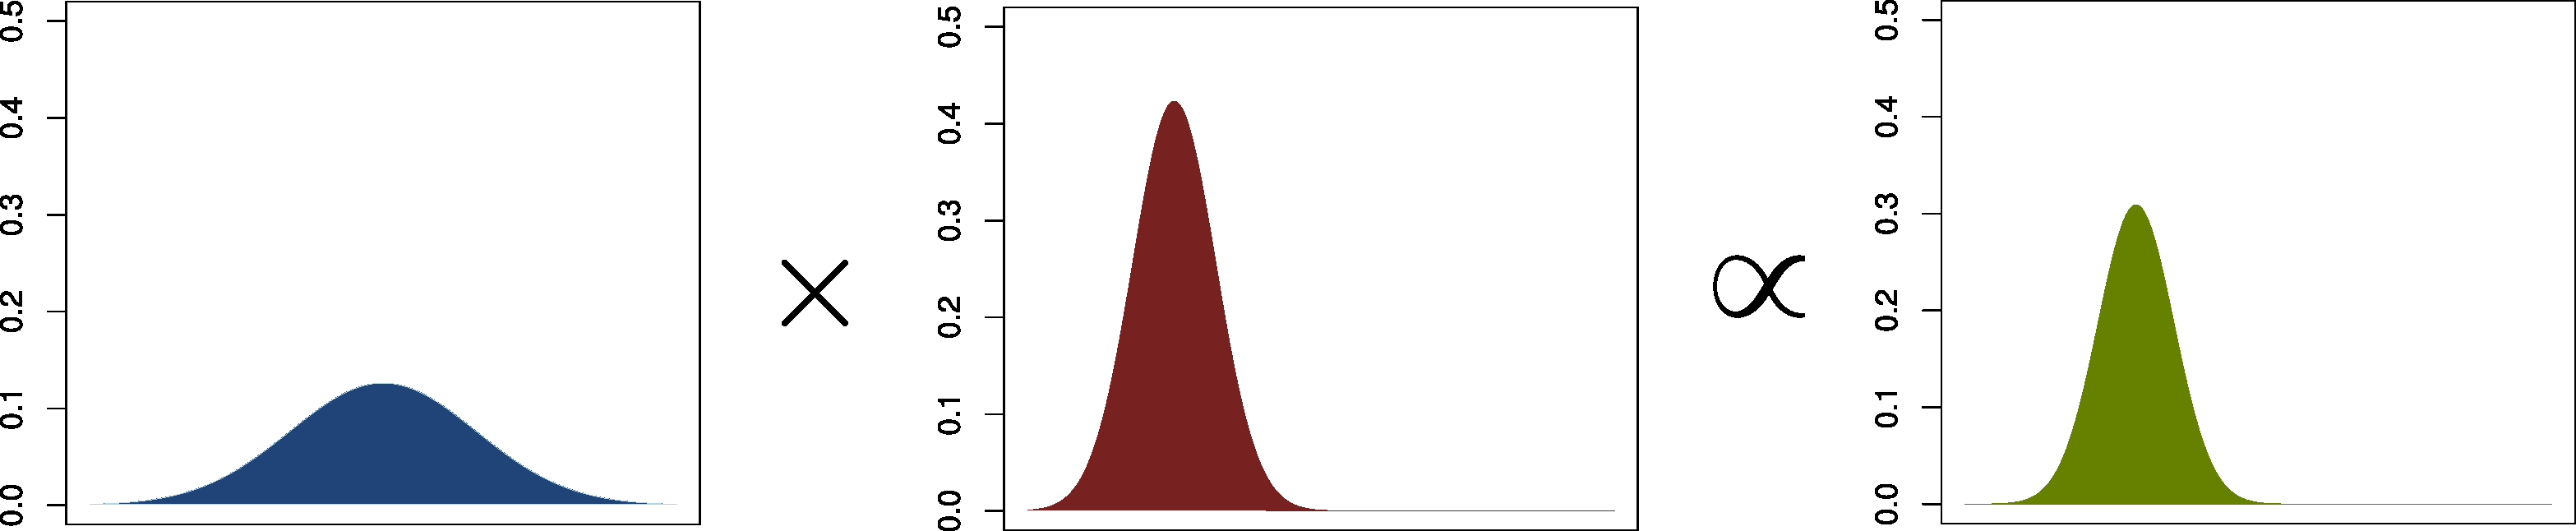
\includegraphics[width=0.7\textwidth]{imgs/bayes_rule.pdf}
        \end{center}
    \end{overprint}
\end{frame}